\chapter{Communication entre robots et supervision (V2X)}
\label{chap:v2x}

La communication V2X constitue l'un des fondements du système \kw{Auto Fleet}. Elle assure la continuité des échanges entre les robots, la station de supervision et les services logiciels qui composent l'infrastructure de contrôle. Dans une flotte mobile, la qualité de ces échanges conditionne directement la réactivité des commandes, la cohérence de l'état affiché, la disponibilité des flux vidéo et la capacité du système à diagnostiquer une situation en cours de mission.

La solution retenue s'appuie sur une architecture distribuée : les fonctions de perception et d'action restent proches des robots, tandis que la supervision centralise l'observation, la coordination et la prise de décision opérateur. Cette séparation permet de conserver des robots autonomes au niveau local, tout en fournissant une vision globale de la flotte. Le système combine ainsi un robot embarqué sur \kw{Raspberry Pi}, un bus de messages \outil{MQTT}, un backend applicatif, une passerelle vidéo, une interface Web de supervision et des modules de perception capables d'intégrer caméra, Kinect, LiDAR et IMU.

\section{Objectifs de la couche V2X}

La couche V2X répond à trois objectifs principaux : transmettre les commandes avec un délai maîtrisé, maintenir une représentation fiable de l'état de la flotte et rendre les flux de perception exploitables par la supervision. Elle joue donc un rôle d'interface entre le monde robotique, fortement contraint par le temps réel et les capteurs, et le monde applicatif, orienté visualisation, diagnostic et interaction utilisateur.

\subsection{Contrat fonctionnel}

Le premier rôle de la couche V2X concerne la \kw{commande}. L'opérateur doit pouvoir sélectionner un robot, changer son mode, envoyer une consigne de téléopération, lancer une mission ou interrompre une action. Ces messages sont courts, mais leur priorité fonctionnelle est élevée. Le système associe chaque commande à un identifiant et à un retour d'exécution, ce qui permet de distinguer une commande reçue, appliquée ou rejetée.

Le deuxième rôle concerne la \kw{télémétrie}. Chaque robot publie périodiquement son état courant : mode, niveau de batterie, pose estimée, vitesse, état réseau, disponibilité des capteurs et horodatage. La supervision ne travaille pas directement sur des messages bruts ; elle consomme une représentation consolidée produite par le backend. Cette consolidation rend l'IHM indépendante du détail des protocoles et facilite l'ajout de nouveaux robots.

Le troisième rôle concerne les \kw{états de service}. Une flotte n'est pas uniquement composée de robots physiques ; elle dépend aussi de services logiciels tels que le broker de messages, le backend, la passerelle vidéo, les modules de perception et les agents embarqués. Le suivi de ces services permet de différencier une perte radio, une indisponibilité caméra, une interruption d'un flux vidéo ou une erreur applicative.

Le quatrième rôle concerne les \kw{flux de perception}. L'image couleur, la profondeur Kinect, les mesures LiDAR et les données IMU n'ont pas toutes la même fréquence, le même volume ou la même criticité. La couche V2X définit donc un format commun pour publier des états synthétiques : disponibilité du capteur, fréquence effective, qualité du signal, mesure minimale pertinente et niveau de confiance. Les données lourdes restent traitées par des modules spécialisés, tandis que la supervision reçoit une information directement exploitable.

\begin{table}[H]
\centering
\small
\renewcommand{\arraystretch}{1.18}
\begin{tabular}{|p{3.4cm}|p{3.0cm}|p{4.5cm}|p{4.0cm}|}
\hline
\textbf{Famille de données} & \textbf{Sens principal} & \textbf{Contenu} & \textbf{Rôle système} \\
\hline
Commandes & station vers robot & mode, téléopération, mission, arrêt & action opérateur et coordination \\
\hline
Télémétrie & robot vers station & batterie, pose, vitesse, état, horodatage & suivi temps réel de la flotte \\
\hline
Accusés de réception & robot vers station & identifiant, statut, délai, message & validation des commandes \\
\hline
États de service & services vers station & backend, broker, vidéo, perception, agent & diagnostic de l'infrastructure \\
\hline
Flux vidéo & robot vers passerelle, puis IHM & RTSP, MJPEG, snapshot & observation visuelle \\
\hline
Synthèse capteurs & robot vers station & caméra, Kinect, LiDAR, IMU, fusion & perception multi-capteurs \\
\hline
Alertes & robot ou backend vers station & obstacle, perte de lien, anomalie, mission & priorisation opérateur \\
\hline
\end{tabular}
\caption{Familles de données échangées dans la couche V2X}
\label{tab:v2x_messages_v2}
\end{table}

\subsection{Contraintes de communication}

Le système évolue sur un réseau local sans fil, donc dans un environnement où la latence, le jitter et la bande passante peuvent varier. L'architecture doit rester robuste lorsque la qualité radio fluctue, lorsque plusieurs flux vidéo sont actifs ou lorsque plusieurs robots publient simultanément leur télémétrie.

La \kw{latence} est critique pour la téléopération. Une commande doit atteindre le robot rapidement et produire un retour mesurable. Le système mesure donc le délai de bout en bout entre l'envoi d'un ordre et la réception de son accusé de réception. Cette mesure fournit une indication plus représentative de l'expérience opérateur qu'une simple latence réseau.

Le \kw{jitter} décrit la régularité des échanges. Dans une interface de supervision, des messages irréguliers peuvent produire des courbes instables et rendre difficile l'interprétation de l'état réel. Le backend maintient donc l'âge des derniers messages, la fréquence effective de réception et l'état de disponibilité de chaque robot.

La \kw{bande passante} concerne principalement la vidéo et les données de perception. Les messages MQTT restent légers, tandis que les flux visuels peuvent devenir coûteux. La passerelle vidéo applique des profils de qualité afin d'adapter la résolution et la compression au contexte d'utilisation. Les débits sont présentés en \kw{KB/s} et \kw{MB/s}, avec une base de calcul de 1024, afin de conserver une lecture homogène dans toute l'IHM.

\begin{table}[H]
\centering
\small
\renewcommand{\arraystretch}{1.18}
\begin{tabular}{|p{3.5cm}|p{5.6cm}|p{4.5cm}|}
\hline
\textbf{Indicateur} & \textbf{Interprétation} & \textbf{Utilisation} \\
\hline
Âge du heartbeat & temps écoulé depuis le dernier signe de vie & statut en ligne ou hors ligne \\
\hline
Latence télémétrie & délai estimé de remontée des données & fraîcheur des informations affichées \\
\hline
RTT commande & délai entre commande et accusé de réception & réactivité opérateur \\
\hline
Jitter & variabilité temporelle des messages & stabilité de la supervision \\
\hline
Débit & volume transféré en KB/s ou MB/s & choix du profil vidéo \\
\hline
Disponibilité vidéo & état du flux caméra et de la passerelle & distinction entre panne vidéo et panne robot \\
\hline
Qualité radio & indication de la robustesse du lien Wi-Fi & anticipation d'une dégradation \\
\hline
\end{tabular}
\caption{Indicateurs utilisés pour qualifier la communication V2X}
\label{tab:v2x_qos_v2}
\end{table}

\section{Architecture de communication}

L'architecture V2X repose sur une séparation nette entre trois niveaux : le niveau embarqué, le niveau applicatif et le niveau d'interface. Le niveau embarqué publie les données issues du robot et reçoit les commandes. Le niveau applicatif consolide les messages, applique les règles de supervision et expose une API stable. Le niveau d'interface présente les informations à l'opérateur et transmet ses décisions au backend.

\subsection{Rôle du backend}

Le backend constitue le point de convergence de la supervision. Il consomme les topics MQTT publiés par les robots et les services, maintient un état courant par robot et expose à l'IHM une structure homogène. Ce choix évite de faire dépendre le navigateur de la topologie MQTT et simplifie la logique d'affichage.

Le backend assure également la cohérence temporelle des données. Chaque message reçu est horodaté, associé à son robot et intégré dans une représentation consolidée. Cette représentation regroupe l'état robot, l'état réseau, les services actifs, la disponibilité vidéo et la synthèse capteurs. L'IHM peut ainsi afficher un état unique sans reconstituer elle-même les messages de bas niveau.

\subsection{Choix de MQTT et articulation avec ROS 2}

\outil{ROS 2} reste adapté aux échanges internes au robot : navigation, perception locale, contrôle et messages capteurs à forte fréquence. \outil{MQTT} est utilisé pour la couche de supervision, car il fournit un mécanisme léger de publication et d'abonnement, bien adapté à la télémétrie, aux états applicatifs et aux commandes de haut niveau.

Cette articulation évite de transformer l'IHM en client direct du middleware robotique. Les robots conservent leur logique embarquée, tandis que la station de supervision reçoit des messages normalisés. L'ajout d'un nouveau robot consiste à publier les mêmes familles de topics avec un nouvel identifiant, sans modifier la structure générale de la supervision.

\begin{table}[H]
\centering
\small
\renewcommand{\arraystretch}{1.18}
\begin{tabular}{|p{4.4cm}|p{4.4cm}|p{5.2cm}|}
\hline
\textbf{Topic logique} & \textbf{Producteur principal} & \textbf{Utilisation} \\
\hline
\texttt{fleet/v1/telemetry/R1} & agent robot & état courant et données réseau \\
\hline
\texttt{fleet/v1/heartbeat/R1} & agent robot & présence et disponibilité \\
\hline
\texttt{fleet/v1/command/R1} & backend & commande de mode, mission ou téléopération \\
\hline
\texttt{fleet/v1/ack/R1} & agent robot & retour sur commande \\
\hline
\texttt{fleet/v1/video\_status/R1} & passerelle vidéo & état du flux, résolution, FPS, débit \\
\hline
\texttt{fleet/v1/sensor/R1} & agent robot & synthèse caméra, Kinect, LiDAR, IMU \\
\hline
\texttt{fleet/v1/heartbeat/backend} & backend & disponibilité de la supervision \\
\hline
\end{tabular}
\caption{Organisation des topics de supervision}
\label{tab:v2x_topics}
\end{table}

\subsection{Découverte et adaptation au réseau}

La supervision intègre une logique de découverte réseau afin de rester exploitable lorsque l'environnement change. Les robots et les services sont identifiés par leur rôle, leur disponibilité et les ports applicatifs qu'ils exposent. La station peut ainsi vérifier la présence d'un robot, qualifier l'accessibilité de ses flux et mettre à jour les endpoints utilisés par la supervision.

Cette capacité est importante pour une flotte mobile, car l'adresse d'un robot peut évoluer selon le réseau utilisé. La découverte ne remplace pas la configuration nominale, mais elle réduit la dépendance à des adresses figées et accélère le retour en service. Elle participe également au diagnostic, en distinguant un robot absent, un service indisponible et un flux vidéo non joignable.

\begin{figure}[H]
    \centering
    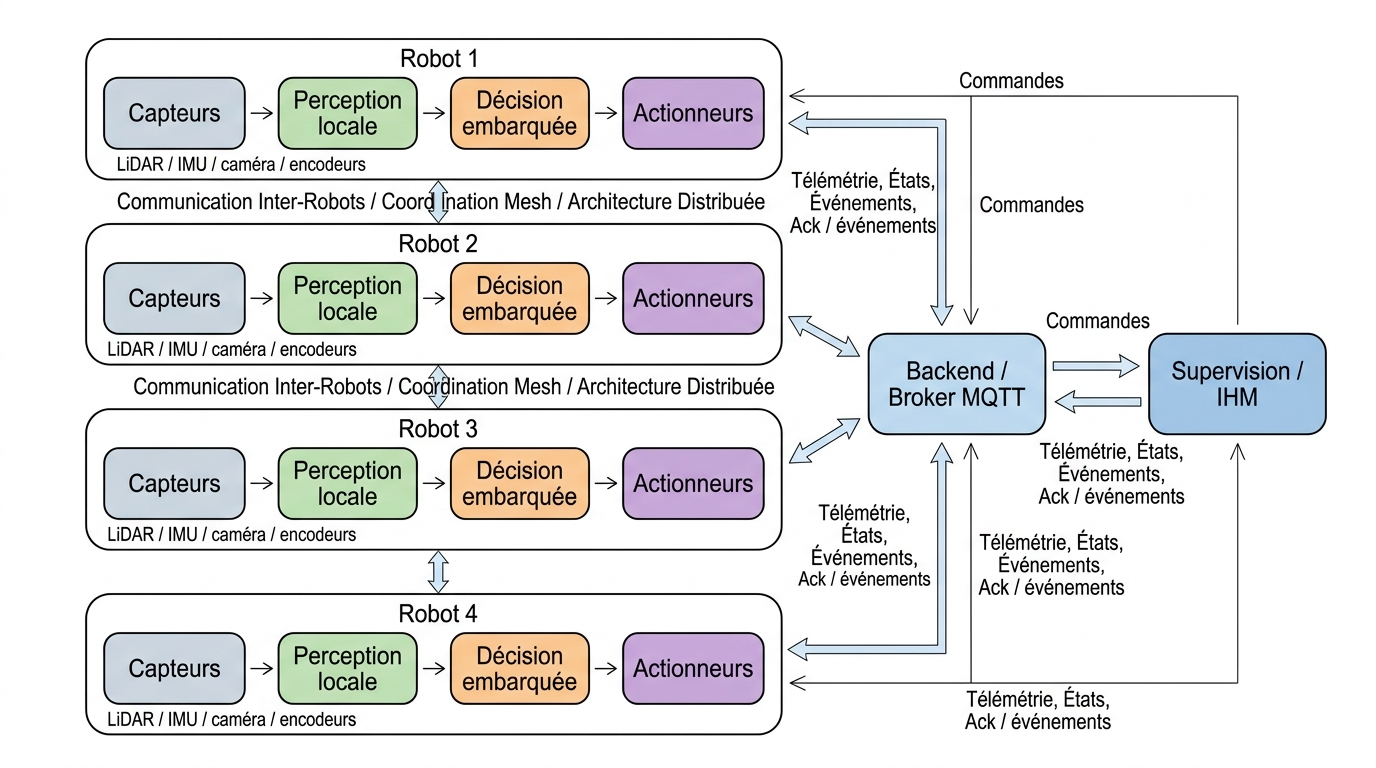
\includegraphics[width=0.92\textwidth]{images/archi_generale_v2.png}
    \caption{Architecture logique de la communication V2X}
    \label{fig:v2x_architecture_logicielle_v2}
\end{figure}

\section{Supervision Web et interaction opérateur}

L'IHM fournit une vue unifiée de la flotte et des services qui la supportent. Elle regroupe le suivi des robots, la téléopération, les commandes de mission, les courbes réseau, l'état vidéo, les alertes et les informations de perception. Son rôle est de rendre la situation exploitable par l'opérateur, sans exposer directement la complexité des flux internes.

\subsection{Vue flotte}

La vue flotte présente chaque robot sous forme de ligne synthétique. Elle affiche l'identifiant, l'état en ligne, le mode courant, la batterie, l'âge du dernier message, la latence, le jitter, le débit, le RTT de commande, la disponibilité vidéo et l'état des capteurs principaux.

Cette approche permet de comparer rapidement plusieurs robots et d'identifier les priorités d'intervention. Un robot peut être disponible pour les commandes mais privé de vidéo ; un autre peut conserver son flux visuel tout en présentant une télémétrie dégradée. La séparation des indicateurs rend ces cas lisibles.

\subsection{Commandes et accusés de réception}

Les commandes opérateur transitent par le backend avant d'être publiées vers le robot cible. Le backend attribue un identifiant à chaque ordre, conserve le contexte d'envoi et attend le retour associé. Le robot publie ensuite un accusé de réception décrivant l'état de la commande.

Ce mécanisme apporte deux garanties. Il permet d'abord à l'IHM d'afficher un retour explicite à l'opérateur. Il permet ensuite de mesurer le temps de réponse réel du robot, en incluant le trajet applicatif complet. Cette mesure sert à qualifier la réactivité de la flotte pendant une mission.

\subsection{Vidéo et profils de qualité}

La vidéo est traitée par une passerelle dédiée. Le robot publie un flux RTSP, puis la passerelle le convertit en MJPEG pour l'affichage Web. Ce choix assure une intégration simple dans le navigateur et maintient la conversion vidéo dans un service isolé, plus facile à surveiller et à adapter.

Quatre profils de qualité sont disponibles. Ils agissent sur la largeur maximale, la qualité JPEG et l'intervalle d'envoi MJPEG. Le profil le plus réactif réduit la résolution afin de minimiser la latence perçue, tandis que les profils de qualité supérieure améliorent la lisibilité lorsque le réseau et la charge processeur le permettent.

\begin{table}[H]
\centering
\small
\renewcommand{\arraystretch}{1.18}
\begin{tabular}{|p{3.2cm}|p{2.3cm}|p{2.5cm}|p{2.8cm}|p{3.6cm}|}
\hline
\textbf{Profil} & \textbf{Largeur max.} & \textbf{Qualité JPEG} & \textbf{Intervalle MJPEG} & \textbf{Usage visé} \\
\hline
Ultra Low Latency & 360 px & 54 & 40 ms & priorité à la réactivité \\
\hline
Balanced & 640 px & 68 & 30 ms & compromis par défaut \\
\hline
Quality & 960 px & 76 & 35 ms & meilleure lisibilité visuelle \\
\hline
High Quality & 1280 px & 82 & 45 ms & observation détaillée \\
\hline
\end{tabular}
\caption{Profils de qualité disponibles pour la vidéo}
\label{tab:v2x_video_profiles}
\end{table}

\subsection{Diagnostic réseau}

Le diagnostic réseau rassemble les mesures de latence, jitter, RTT, perte et débit. Les valeurs de débit sont affichées de manière homogène en KB/s ou MB/s. Cette présentation correspond à la lecture attendue par l'opérateur pour des volumes de données, notamment les flux vidéo.

La supervision peut également estimer la charge induite par plusieurs flux simultanés. Cette estimation aide à déterminer si la priorité doit être donnée à la qualité visuelle ou à la réactivité. Elle prépare aussi le passage à une flotte plus grande, où l'affichage de toutes les vidéos en haute qualité ne constitue pas toujours le meilleur choix opérationnel.

\begin{figure}[H]
    \centering
    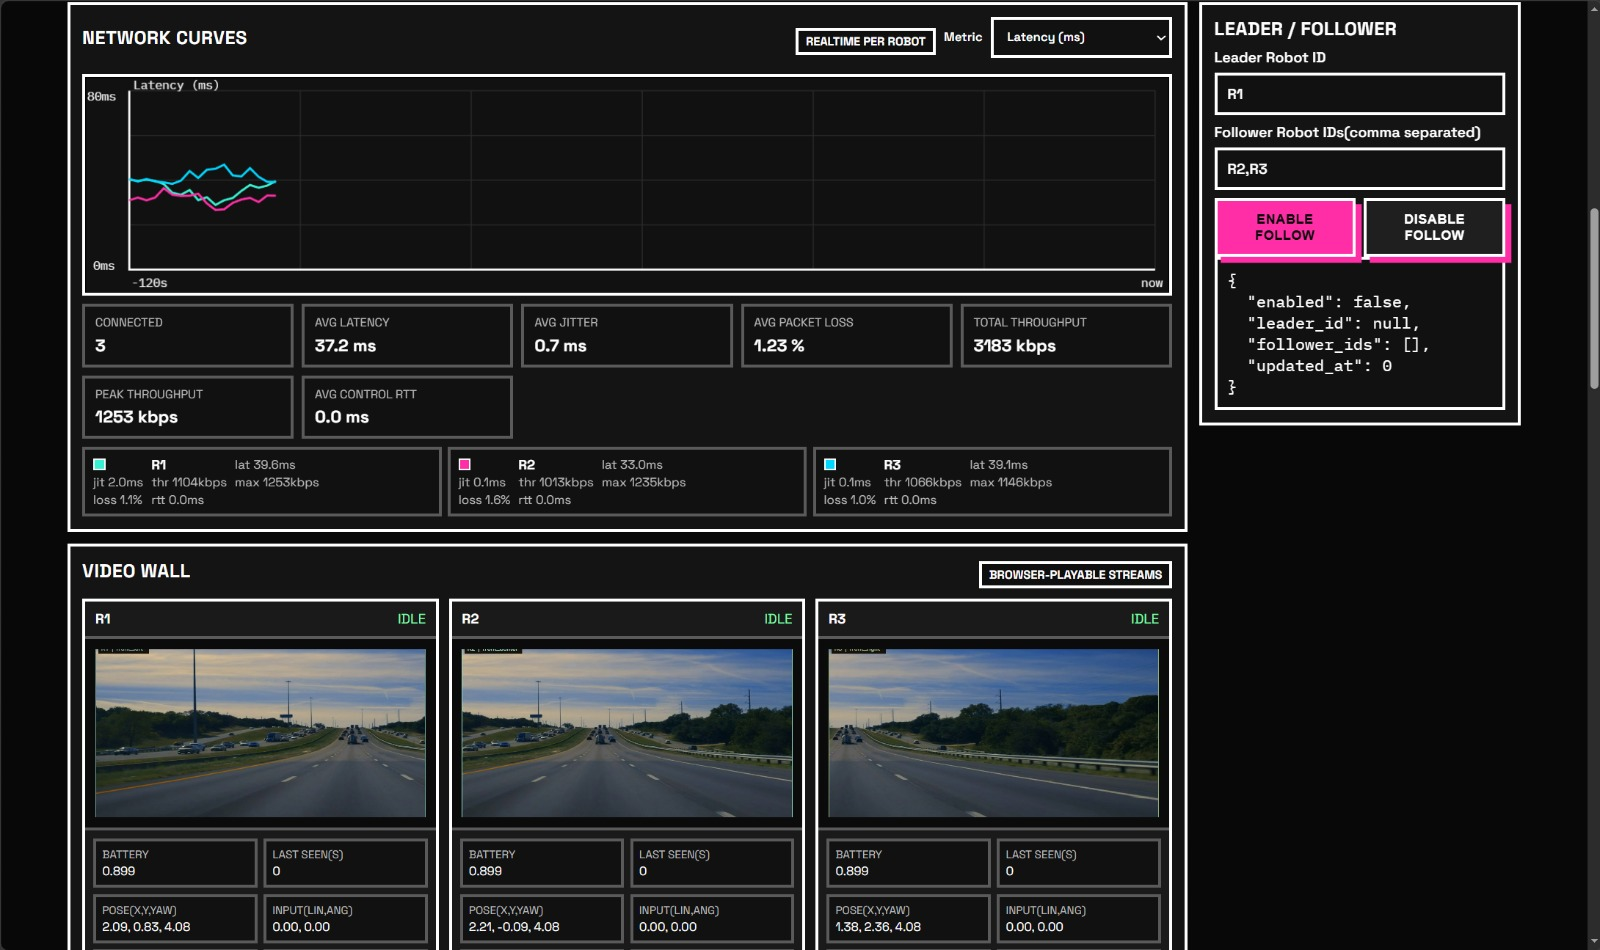
\includegraphics[width=0.92\textwidth]{images/baba.png}
    \caption{Organisation générale de l'IHM de supervision}
    \label{fig:v2x_ihm_generale_v2}
\end{figure}

\section{Intégration robot et perception multi-capteurs}

Le robot R1 représente l'implémentation complète de la chaine V2X sur une plateforme réelle. Il associe un agent embarqué, une caméra, un flux vidéo, une télémétrie MQTT et des états capteurs publiés vers la supervision. Cette intégration valide le passage d'une architecture logicielle à une chaine robotique observable et commandable.

\subsection{Agent embarqué}

L'agent embarqué joue le rôle d'adaptateur entre le robot et la supervision. Il publie la télémétrie, les heartbeats, les accusés de réception et la synthèse capteurs. Il reçoit les commandes de haut niveau et les transmet aux fonctions locales du robot.

Cette séparation permet de garder une frontière claire entre la logique embarquée et la supervision. Les traitements bas niveau restent du côté robot, tandis que la station reçoit des états normalisés. La même structure peut être reproduite sur d'autres robots de la flotte.

\begin{table}[H]
\centering
\small
\renewcommand{\arraystretch}{1.18}
\begin{tabular}{|p{4.0cm}|p{6.0cm}|p{3.6cm}|}
\hline
\textbf{Élément} & \textbf{Fonction} & \textbf{Rôle V2X} \\
\hline
Agent robot & publication MQTT et réception des commandes & interface embarquée \\
\hline
Caméra RGB & acquisition visuelle et flux RTSP & observation vidéo \\
\hline
Kinect & profondeur et estimation de distance & perception 3D \\
\hline
LiDAR & distances et obstacles & navigation et sécurité \\
\hline
IMU & orientation et mouvements & stabilisation et diagnostic \\
\hline
Backend & agrégation des messages & état consolidé \\
\hline
IHM & affichage et interaction & supervision opérateur \\
\hline
\end{tabular}
\caption{Rôle des composants dans l'intégration V2X de R1}
\label{tab:v2x_r1_integration}
\end{table}

\subsection{Chaîne vidéo}

La chaîne vidéo relie l'acquisition embarquée à l'affichage Web. La caméra produit un flux sur le robot, ce flux est publié en RTSP, puis converti par la passerelle en MJPEG. La supervision reçoit en parallèle l'état du flux : disponibilité, résolution, fréquence, débit et URL de snapshot.

Ce découpage isole les responsabilités. Le robot se concentre sur l'acquisition et la publication du flux. La passerelle gère la conversion et les profils de qualité. Le navigateur affiche un format simple, compatible et léger à intégrer. Cette organisation limite le couplage entre matériel caméra, protocole vidéo et interface utilisateur.

\subsection{Synthèse capteurs}

La supervision ne se limite pas à l'image RGB. La Kinect fournit une information de profondeur exploitable pour estimer les distances et enrichir l'analyse de l'environnement. Le LiDAR apporte une mesure de distance plus adaptée à la détection d'obstacles et à la cartographie. L'IMU complète ces informations par l'orientation, les accélérations et la détection de mouvements brusques.

Les données capteurs sont ramenées à une synthèse commune avant affichage. Pour chaque capteur, le message indique l'état, la fréquence, la dernière mise à jour, la mesure principale et un niveau de confiance. Cette approche évite de saturer l'IHM avec des données brutes et fournit à l'opérateur des informations directement interprétables.

\begin{figure}[H]
    \centering
    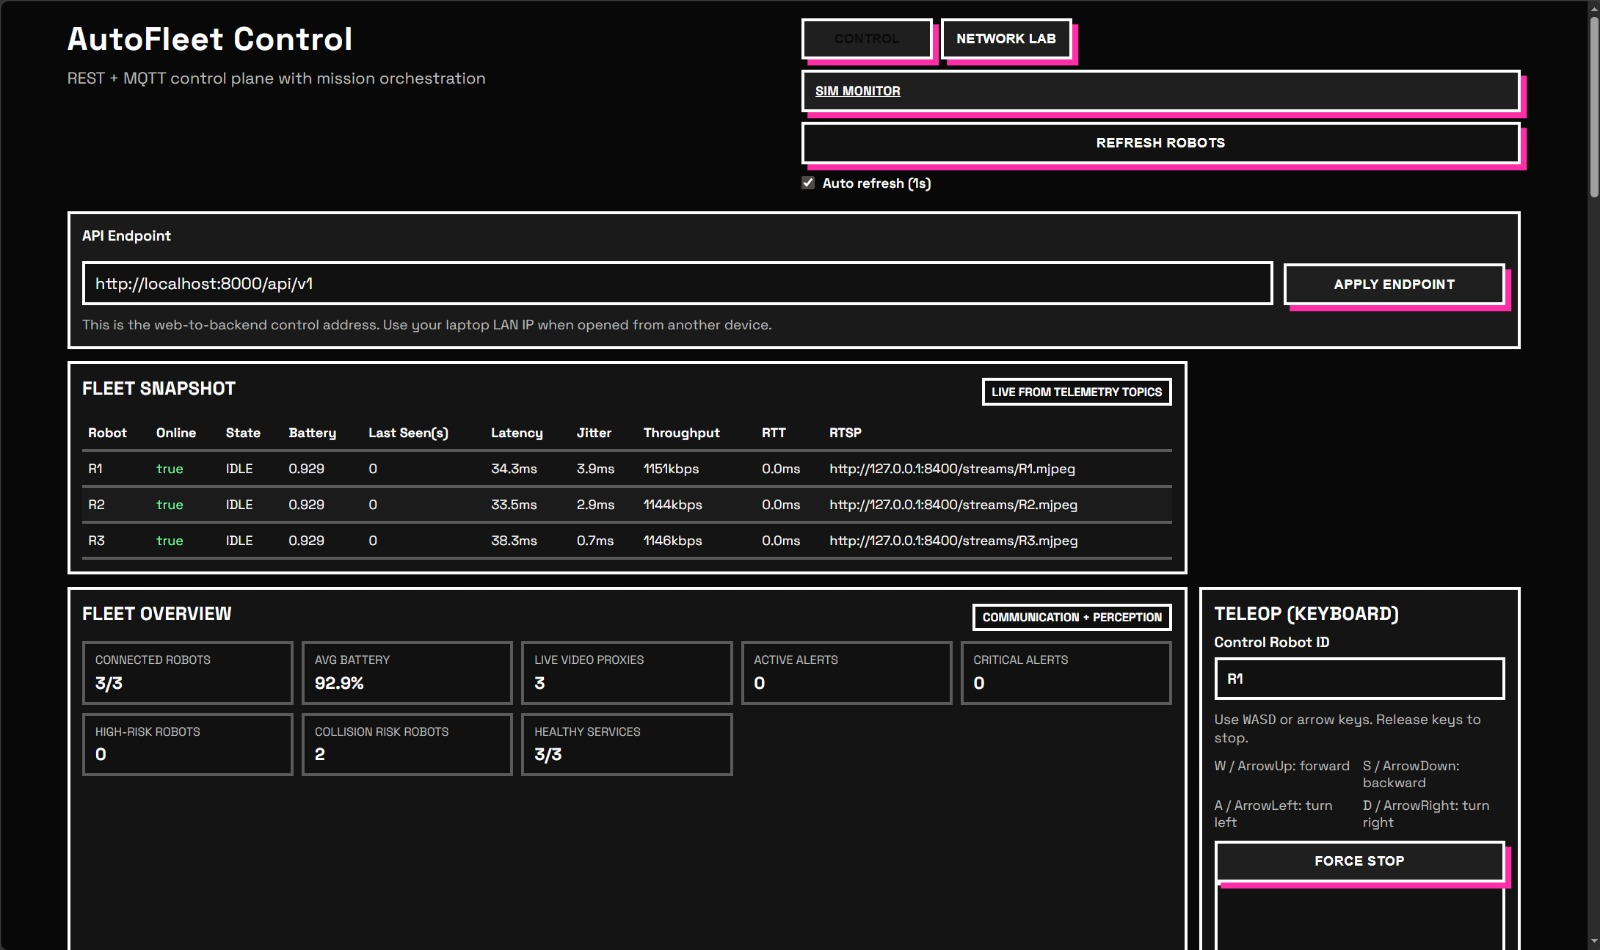
\includegraphics[width=0.92\textwidth]{images/7.jpg}
    \caption{Vue de diagnostic réseau et de gestion des flux vidéo}
    \label{fig:v2x_diagnostic_reseau_v2}
\end{figure}

\section{Validation de l'architecture}

La validation de la couche V2X s'appuie sur la cohérence entre les messages publiés, l'état consolidé côté backend et l'affichage dans l'IHM. Le système est validé lorsque les commandes, la télémétrie, la vidéo, les états de service et la synthèse capteurs restent cohérents dans la supervision.

\subsection{Résultats obtenus}

La chaine réalisée permet à la station de recevoir la télémétrie de R1, d'envoyer des commandes, de mesurer les délais de réponse, d'afficher le flux vidéo et de présenter l'état des capteurs. Les indicateurs réseau sont visibles dans l'IHM, les débits sont exprimés en KB/s ou MB/s et les profils vidéo peuvent être appliqués à l'ensemble des robots affichés.

Ces résultats valident l'architecture retenue : le backend joue son rôle de couche de consolidation, MQTT fournit un transport léger pour la supervision, la passerelle vidéo rend le flux exploitable par le navigateur et l'IHM présente une lecture unifiée de la flotte.

\subsection{Scalabilité}

L'architecture est conçue pour évoluer vers plusieurs robots. Les topics utilisent un identifiant robot, les états sont maintenus par entité et les profils vidéo s'appliquent de manière homogène. L'ajout d'un robot revient donc à ajouter une nouvelle instance de publication respectant le même contrat de messages.

La supervision peut ensuite hiérarchiser l'affichage selon le nombre de robots : vue synthétique pour la flotte, détails à la demande, priorisation des alertes et adaptation des flux vidéo. Cette logique évite que l'augmentation du nombre de robots se traduise par une surcharge directe de l'interface.

\subsection{Perspectives d'évolution}

Les évolutions principales concernent l'adaptation dynamique. Le système peut ajuster automatiquement le profil vidéo selon la latence, le débit disponible et la charge CPU. Les informations Kinect, LiDAR et IMU peuvent également être fusionnées pour produire une perception plus riche : distance minimale, obstacle prioritaire, orientation, stabilité et confiance globale.

Une évolution vers WebRTC peut être envisagée pour les scénarios où la latence vidéo devient prioritaire. Cette évolution ne modifie pas le principe d'architecture : le robot publie un flux, une passerelle spécialisée l'adapte et l'IHM consomme une représentation compatible avec le Web.

\begin{table}[H]
\centering
\small
\renewcommand{\arraystretch}{1.18}
\begin{tabular}{|p{3.4cm}|p{5.4cm}|p{5.0cm}|}
\hline
\textbf{Axe} & \textbf{Réalisation} & \textbf{Évolution} \\
\hline
Réseau & découverte, heartbeat, mesure RTT & sélection automatique du meilleur chemin \\
\hline
Vidéo & RTSP vers MJPEG, profils qualité & adaptation dynamique et WebRTC \\
\hline
Capteurs & caméra, Kinect, LiDAR, IMU & fusion multi-capteurs \\
\hline
Supervision & vue flotte, commandes, diagnostic & priorisation et historique enrichi \\
\hline
Scalabilité & topics par robot, état consolidé & orchestration multi-robots avancée \\
\hline
\end{tabular}
\caption{Synthèse de la validation et des évolutions V2X}
\label{tab:v2x_perspectives}
\end{table}

En conclusion, la couche V2X fournit l'infrastructure de communication nécessaire à une flotte supervisée. Elle relie les robots, les services applicatifs, les flux vidéo et les capteurs dans une architecture cohérente. Cette base permet d'assurer la commande, l'observation, le diagnostic et l'extension multi-capteurs du système \kw{Auto Fleet}.
